%!TEX root = ../Thesis.tex

\section{Skip-gram}

The Skip-gram model tries to learn the meaning of words by its context. Specifically it tries to predict the surrounding words a given a single input word. This is different from CBOW \todo{shold this be discusessed}, because only one word is used as input and multiply words are used as output.

\begin{figure}[H]
	\centering
	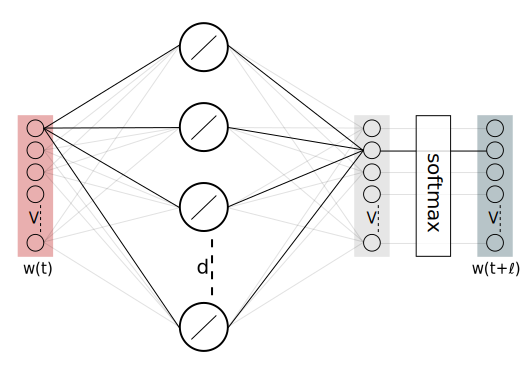
\includegraphics[width=0.8\textwidth]{theory/skip-gram}
	\caption{Visualization of a single pass though the Skip-gram network. Note that there are no non-linear units, thus this is a log-linear method.}
\end{figure}

The model is optimized by maximum-likelihood over all the words ($w_t, t \in [1, T]$) \todo{boundary issue} as input and to some of the surrounding words ($w_{t + \ell}$):
\begin{equation}
\mathcal{L} = \prod_{t = 1}^T \prod_{\ell} p(w_{t + \ell} | w_t)
\end{equation}

Since words closer to $w_t$ should be more related to that word, the near surrounding words are weighed higher. This is done by letting $\ell \in [-R, R] \setminus \{ 0 \}$ where $R \sim U[1, C]$ \cite{word2vec-comparing}.

For easier calculation of $\mathcal{L}$, the average log likelihood is used instead:
\begin{equation}
\frac{1}{T} \log( \mathcal{L} ) = \frac{1}{T} \sum_{t = 1}^T \sum_{\ell} \log( p(w_{t + \ell} | w_t) )
\end{equation}

The words $w$ are represented using 1-of-V encoding\todo{explain}, where $V$ is the vocabulary size. For a given word $w$ this encoding will be denoted as $\mathbf{x}_w$ \todo{Confusing? $x$ indicates input}. The hidden layer (latent representation) is then calculated as:
\begin{equation}
\mathbf{v}_w = \mathbf{x}_w \mathbf{W}^{(1)}
\end{equation} \todo{Introduce weights $W^{(1)}$ and $W^{(2)}$.}

The probability $p(w_{t + \ell} | w_t)$ can now be calculated as:
\begin{equation}
p(w_{t + \ell} | w_t) = p(w_O | w_I) = \mathbf{x}_{w_O}^T \frac{
	\mathbf{exp}(\mathbf{v}_{w_I}  \mathbf{W}^{(2)} )
}{
	\sum_{k=1}^V \mathbf{exp}_k(\mathbf{v}_{w_I}  \mathbf{W}^{(2)} )
}
\end{equation}
\todo{This does not match the paper \cite[eq. 2]{word2vec-details}}

This calculation is problematic since it involves a sum over all words in the vocabulary. In the Skip-gram model the vocabulary can be of size $10^5$ to $10^7$ \cite{word2vec-details} \todo{check this}.
